\documentclass[11pt]{article}

\usepackage{xeCJK}
\usepackage{graphicx}
\usepackage{amsmath}
\usepackage{booktabs}
\usepackage{float}

\setCJKmainfont[BoldFont=SourceHanSerifSC-Bold]{SourceHanSerifSC-Regular}
\setCJKsansfont[BoldFont=SourceHanSansSC-Bold]{SourceHanSansSC-Regular}
\setCJKmonofont{STFangsong}

\renewcommand{\baselinestretch}{1}

\title{OSH调研报告\\[2ex]文件多路传输系统}
\author{吴永基 PB16001676\\黄子昂 PB16001840\\金朔苇 PB16001696\\徐直前 PB16001828}
\date{\today}

\begin{document}
\maketitle
\tableofcontents

\section{项目背景}
随着时代的发展,万物互联的时代即将到来。
而在这样一个时代中,数据处于一个核心的地位,数据成为了一种壁垒,大企业的优势其实就在于数据,
他们利用这些数据训练算法,掌握用户信息,给用户提供定制化的服务。
很多初创小企业因为数据积累的不够,导致算法训练难以收敛,无法与大企业进行有效的竞争。
我们甚至可以得出这样的结论:有数据则生,无数据则死。而在积累了大量的数据后,
如何有效地将这些数据加以利用,进行存储,如何高效地传输则是一个相当大的问题。
在这里我们小组就专门针对高效传输这一问题进行了研究。如果可以解决这个问题,那么我们就可以极高的提高生产效率,
如果从经济学上来考虑,我们相当于极大地降低了“交易成本”,促进了信息之间的更加高效地流通。
使得用户之间信息的传递变得极为方便。
\\
Kevin Kelly在他的著作《必然》中提出过这样一个概念“流动”。
他认为“流动”是未来社会的必然趋势。在未来的商业社会中人们所做的所有生意,都是数据。
计算机中的几个大阶段:原来是文件夹,之后是网络,现在我们处于一个数据流动的时代。
现在的阶段就是流标签,云端组成各种各样的流,通过微信、微博、Facebook等等,我们可以听流媒体上的音乐,看流媒体上的电影电视,
所有东西都成为一种流。什么东西在流动呢?就是数据,不管你是做房地产、医药、化工,还是教育,
其实未来人们做的生意都是数据。商业乃数据之商业。归根结底,人们在处理的都是数据。处理数据和处理客户一样重要。
全世界都处于同一个经济脉搏,企业不可能永远增长。但是城市不一样,城市永远在增长。因特网像一个城市,而不是一个企业,
正因为它拥有着无限增长的特质。比如Facebook现在有15亿的社交连接,15亿人相互连接可以做的事情太多太多了,可以产生的价值也不可估量。很多公司已经意识到了这一点。这么多的数据像是形成了超级生物体,远远超过人脑的容量了,这样一个巨大的机器星球,其实是全球化的一个运作,全世界的经济好像都以同样的脉搏在跳动,以同样的行为方式在运作。
\\
我们平时在使用Wi-Fi、以太网、蜂窝网络、蓝牙等方式传输文件时,仅能同时使用其中的一种方式进行文件的传输。在此情况下,其他设备都处于空闲状态,极大的浪费了资源。而如果能同时利用例如Wi-Fi、以太网、蓝牙等途径传输文件,那么网络的吞吐量(throughput)和健壮性(robustness)都能得到极大的提高。本项目即致在构建一种多路文件传输的实现方式,同时利用多种链路,大幅提高文件传输的速度和稳定性。
本文首先简要介绍一下各种链路的主要使用场景、优缺点。
\subsection{Wi-Fi}
\subsubsection{简介}
\begin{figure}[H]
    \begin{center}
    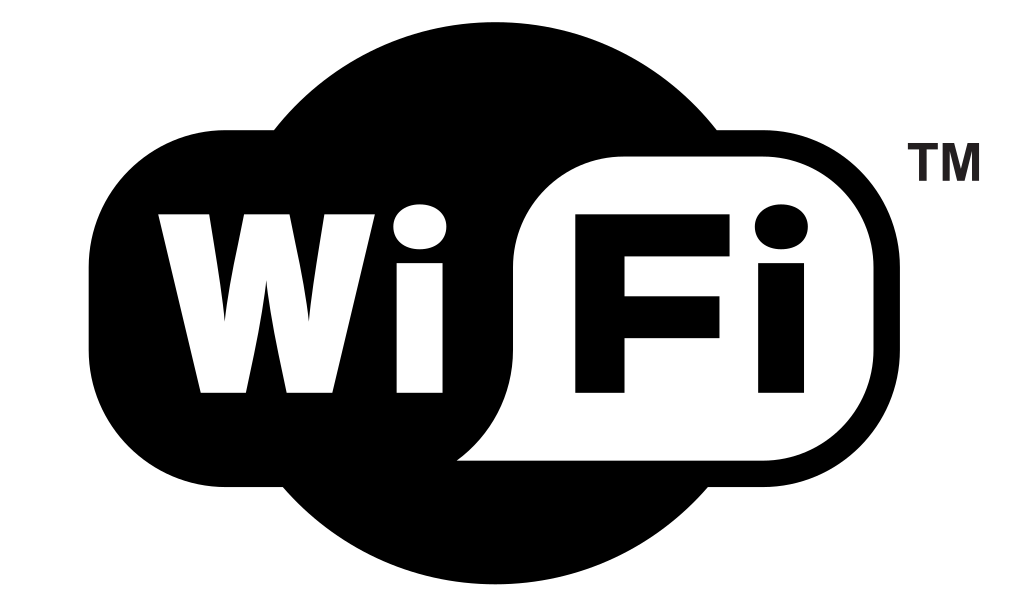
\includegraphics[width=0.67\textwidth]{figures//wifi_logo.png}
    \caption{Wi-Fi}
    \end{center}
\end{figure}
Wi-Fi 是Wi-Fi联盟制造商的商标作为产品的品牌认证,是一个创建于IEEE 802.11标准的无线局域网技术。
Wi-Fi兼容设备通过无线局域网(WLAN)和无线接入点(WAP)连接因特网。这些无线接入点通常在室内有着20m的作用范围。
Wi-Fi通常使用2.4 GHz波段或5.8 GHz波段。它的目标在于改善先前的两项无线网络标准,包括802.11a与802.11g,在网络流量上的不足。它的最大传输速度理论值为600Mbit/s
\subsubsection{IEEE 802.11标准}
IEEE 802.11标准是现今WLAN通用的标准,它定义了媒体访问控制层(MAC layer)和物理层上的一组WLAN实现规格。
这种通讯协议通常工作在900 MHz和2.4, 3.6, 5, 60 GHz。第一个IEEE 802.11标准制定于1997年(IEEE 802.11-1997),
在2.4G ISM频段上实现了1Mbps和2Mbps两种传输速率。并且随后迅速发转,如今已经发展出了一系列不同的协议。
下面将介绍一下现今常见的几种协议。
\begin{enumerate}
    \item IEEE 802.11n
    \item IEEE 802.11ac
    \item IEEE 802.11ad
\end{enumerate}
\paragraph{IEEE 802.11n}
IEEE 802.11n-2009是对IEEE 802.11-2007标准的修正规格,于2009年十月发布。
它的目标在于改善先前的两项无线网络标准,包括802.11a与802.11g,在网络流量上的不足。它的最大传输速度理论值为600Mbit/s。
\\
\textbf{特点}
\begin{itemize}
    \item 802.11n增加了对于MIMO的标准,使用多个发射和接收天线来允许更高的数据传输率,并使用了Alamouti于1998年提出的空时分组码来增加传输范围。
    \item 802.11n支持在标准带宽(20MHz)上的速率包括有(单位Mbit/s):7.2, 14.4, 21.7, 28.9, 43.3, 57.8, 65, 72.2(短保护间隔,单数据流)。使用4xMIMO时速度最高为300Mbit/s。
    \item 802.11n也支持双倍带宽(40MHz),当使用40MHz带宽和4*MIMO时,速度最高可达600Mbit/s。
\end{itemize}
\paragraph{IEEE 802.11ac}
IEEE 802.11ac 标准于2014年1月发布,这项标准仅工作在5GHz频带上,皆在通过5GHz频带提供高通量的无线局域网,
俗称5G WiFi (5th Generation of Wi-Fi)。理论上它能提供最少1Gbps带宽进行多站式WLAN通信,或者500Mbps单一的连接传输带宽。
802.11ac是802.11n的继承者。它采用并扩展了802.11n的空中接口概念。
\\
\textbf{特点}
\begin{itemize}
    \item 扩展绑定的频道
    \begin{itemize}
        \item  强制支持至80MHz带宽(相对于802.11n支持至40MHz带宽),而160MHz带宽为可选择是否支持
    \end{itemize}
    \item 更多的MIMO空间流
    \begin{itemize}
        \item 支持8个MIMO空间流(802.11n只能支持4个)
    \end{itemize}
    \item Downlink Multi-user MIMO \textit{(MU-MIMO)}
    \item 调变 (Modulation)
    \begin{itemize}
        \item 256-QAM, rate 3/4 与 5/6, 可作为选项 (802.11n 最高到达 64-QAM, rate 5/6) 
    \end{itemize}
\end{itemize}
\paragraph{IEEE 802.11ad}
IEEE 802.11ad标准于2013年1月发布,同时支持2.4/5/60 GHz频带,
由WiGig(无线千兆联盟)推动。WiGig三频段设备可以在2.4GHz、5GHz和60GHz频段上工作,
最高可以以7Gbit/s的速度传输数据。
\\
\textbf{特点}
\begin{itemize}
    \item 支持最高 7 Gbit/s的数据传输
    \item 支持并扩展了802.11 MAC层并且和802.11标准向下兼容
    \item 物理层允许低功耗高性能的WiGig设备,保证了互操性和Gigabit/s的速度传输
    \item WiGig设备使用了高级安全和电源管理技术
    \item 支持波束赋形 (beamforming)
\end{itemize}
\subsubsection{Wi-Fi的性能}
\begin{figure}[H]
    \begin{center}
    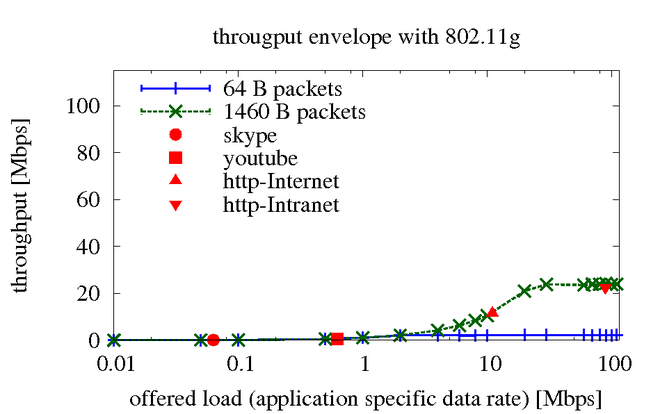
\includegraphics[width=0.67\textwidth]{figures//performance_11g.png}
    \caption{IEEE 802.11g标准, 2.4GHz波段下UDP协议的性能}
    \end{center}
\end{figure}
\begin{figure}[H]
    \begin{center}
    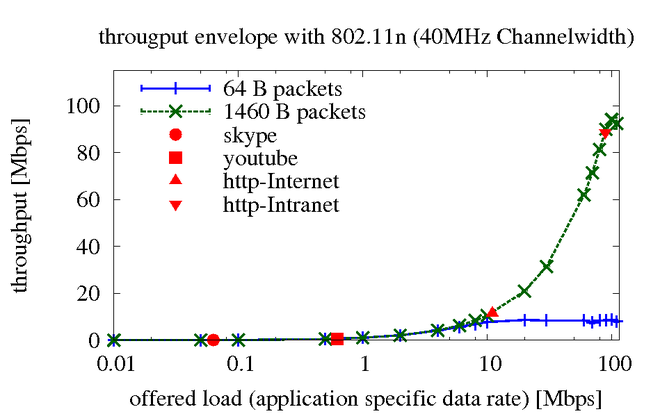
\includegraphics[width=0.67\textwidth]{figures//performance_11n.png}
    \caption{IEEE 802.11n标准40MHz, 2.4GHz波段下UDP协议的性能}
    \end{center}
\end{figure}
\begin{figure}[H]
    \begin{center}
    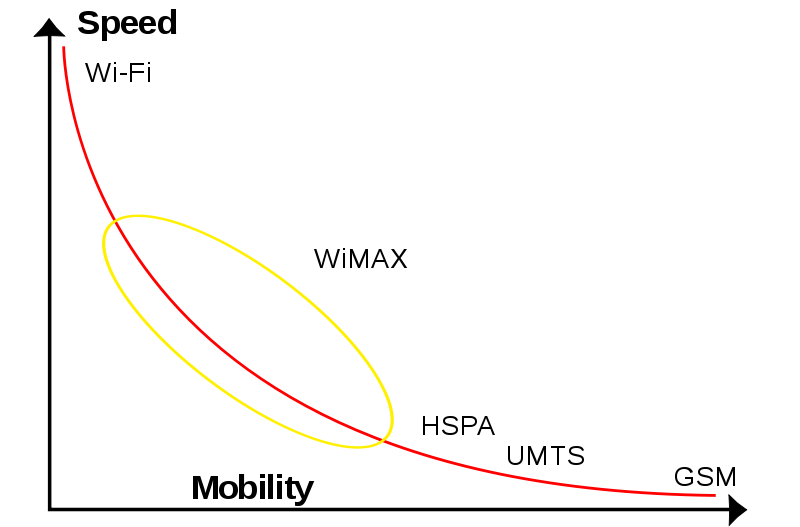
\includegraphics[width=0.67\textwidth]{figures//wifi_comparison.png}
    \caption{传输速度和移动性对比}
    \end{center}
\end{figure}
一个使用802.11b或802.11g的典型无线路由器和天线,
在无任何障碍物下可覆盖范围可达到室内50平方米/室外140平方米。
802.11n可到达超过这个范围两倍的距离,范围随频率的波段调整。
Wi-Fi在2.4 GHz的频率区块范围比5 GHz的频率区块稍微好些。 通过使用定向天线,室外覆盖范围可提高数公里或以上。
\subsection{以太网}
\subsubsection{简介}
以太网(Ethernet)是一种计算机局域网技术。
IEEE组织的IEEE 802.3标准制定了以太网的技术标准,
它规定了包括物理层的连线、电子信号和介质访问层协议的内容。
以太网的标准拓扑结构为总线型拓扑,但目前的快速以太网(100BASE-T、1000BASE-T标准)为了减少冲突,
将能提高的网络速度和使用效率最大化,使用交换机(Switch hub)来进行网络连接和组织。
如此一来,以太网的拓扑结构就成了星型;但在逻辑上,
以太网仍然使用总线型拓扑和CSMA/CD(Carrier Sense Multiple Access/Collision Detection,即载波多重访问/碰撞侦测)
的总线技术。
\subsubsection{Ethernet常见带宽}
\begin{itemize}
    \item{10 Mbps}
    \item{100 Mbps}
    \item{1 Gbps}
    \item{10 Gbps}
    \item{100 Gbps}
\end{itemize}
目前在日常应用中,以1Gbps Ethernet最为常见。
\subsection{蜂窝网络}
\subsubsection{简介}
蜂窝网络(英语:Cellular network),又称移动网络(mobile network)是一种移动通信硬件架构,分为模拟蜂窝网络和数字蜂窝网络。由于构成网络覆盖的各通信基地台的信号覆盖呈六边形,从而使整个网络像一个蜂窝而得名。
常见的蜂窝网络类型有:GSM网络(有些国家叫pcs-1900)、CDMA网络、3G网络、TDMA、PDC、TACS、AMPS等。
蜂窝网络的组成:蜂窝网络组成主要有以下三部分:移动站,基站子系统,网络子系统。移动站就是我们的网络终端设备,比如手机或者一些蜂窝工控设备 。基站子系统包括我们日常见到的移动基站(大铁塔)、无线收发设备、专用网络(一般是光纤)、无数的数字设备等等的。我们可以把基站子系统看作是无线网络与有线网络之间的转换器。
\subsubsection{5G}
\begin{figure}[H]
    \begin{center}
    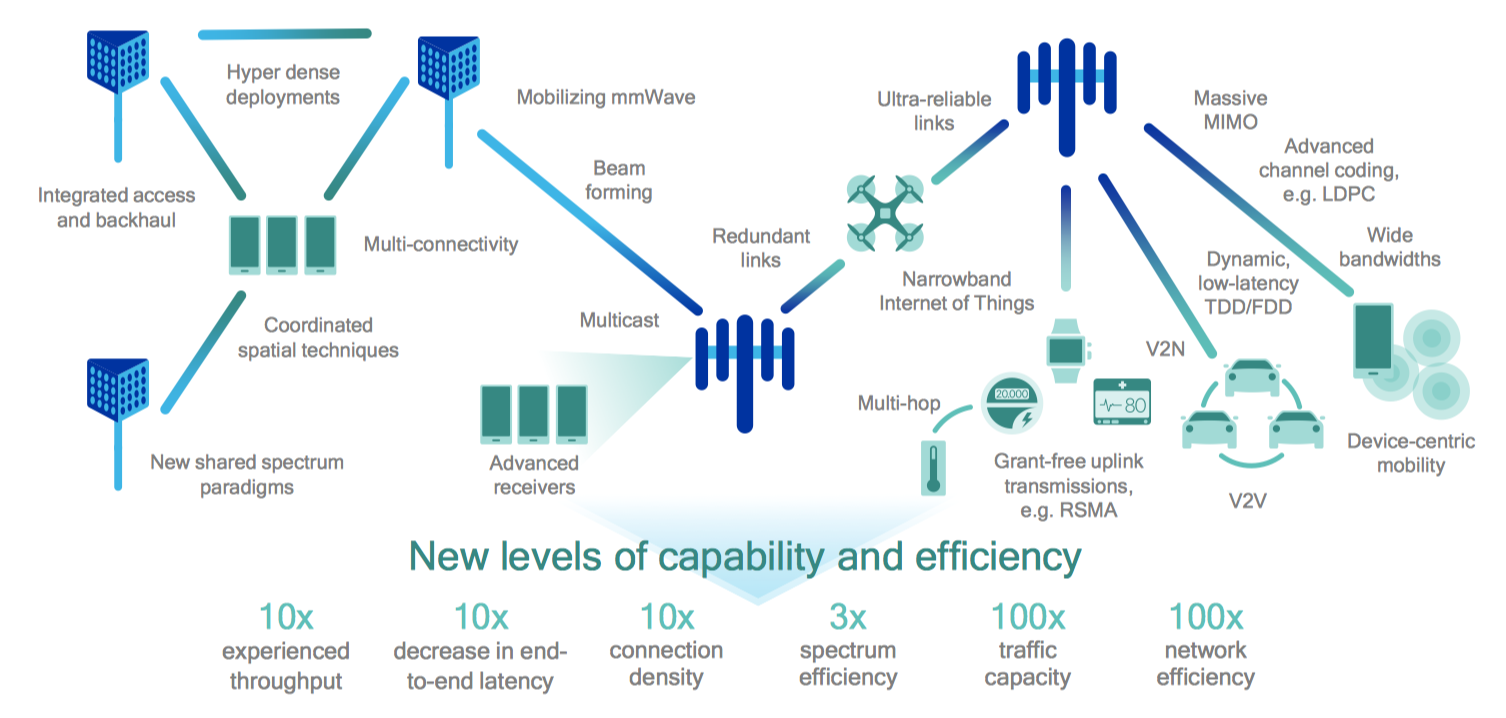
\includegraphics[width=\textwidth]{figures//5g_tech.png}
    \caption{5G核心技术}
    \end{center}
\end{figure}
\paragraph{增强型移动宽带 (EMBB)}
增强型移动宽带的两个关键方面将在5G经济中促进普及和价值创造。
第一个方面是将蜂窝覆盖扩展到范围更广的建筑物中,
包括办公楼、工业园区、购物中心和大型场所。
第二个方面是提升容量以满足使用大量数据的更多终端的需求,尤其在局部地区。
这些网络的改进将支持更高效的数据传输,降低每比特数据传输成本,从而驱动在移动网络中更多地使用宽带应用。
\paragraph{海量物联网 (MIoT)}
5G将利用早前在机器对机器(M2M)和传统物联网(IoT)应用方面的投入,
支持规模经济的显著提升以促进其在全部行业中普及和应用。5G能更好地满足低功耗需求,
实现在授权和非授权频谱工作并提供更深入 更灵活的覆盖,从而在海量物联网情景中显著降低成本。
这亦将支持海量物联网扩大规模,并且将促进海量物联网应用更多地采用移动技术。
\paragraph{关键业务型服务 (MCS)}
关键业务型服务代表移动技术的全新市场机会,
这将是5G重要的增长领域,并将支持那些需要高可靠、超低时延连接以及高安全性与高可用性的应用。
这将支持无线技术提供与有线难以区分的超可靠连接以支持零容错应用,例如自动驾驶汽车和远程操作复杂的自动化设备。
\paragraph{总结}
5G技术将创造一个万物互联的时代,可以提供高网络容量、高速率(数Gbps的峰值速率),提供低能耗、高稳定性、高安全性、极高的用户移动性、高网络密度等特性。
如果能够整合蜂窝数据进入这一多链路传输系统,将会极大提高文件传输的throughput,具有重大意义。
\subsubsection{性能}
\begin{figure}[H]
    \begin{center}
    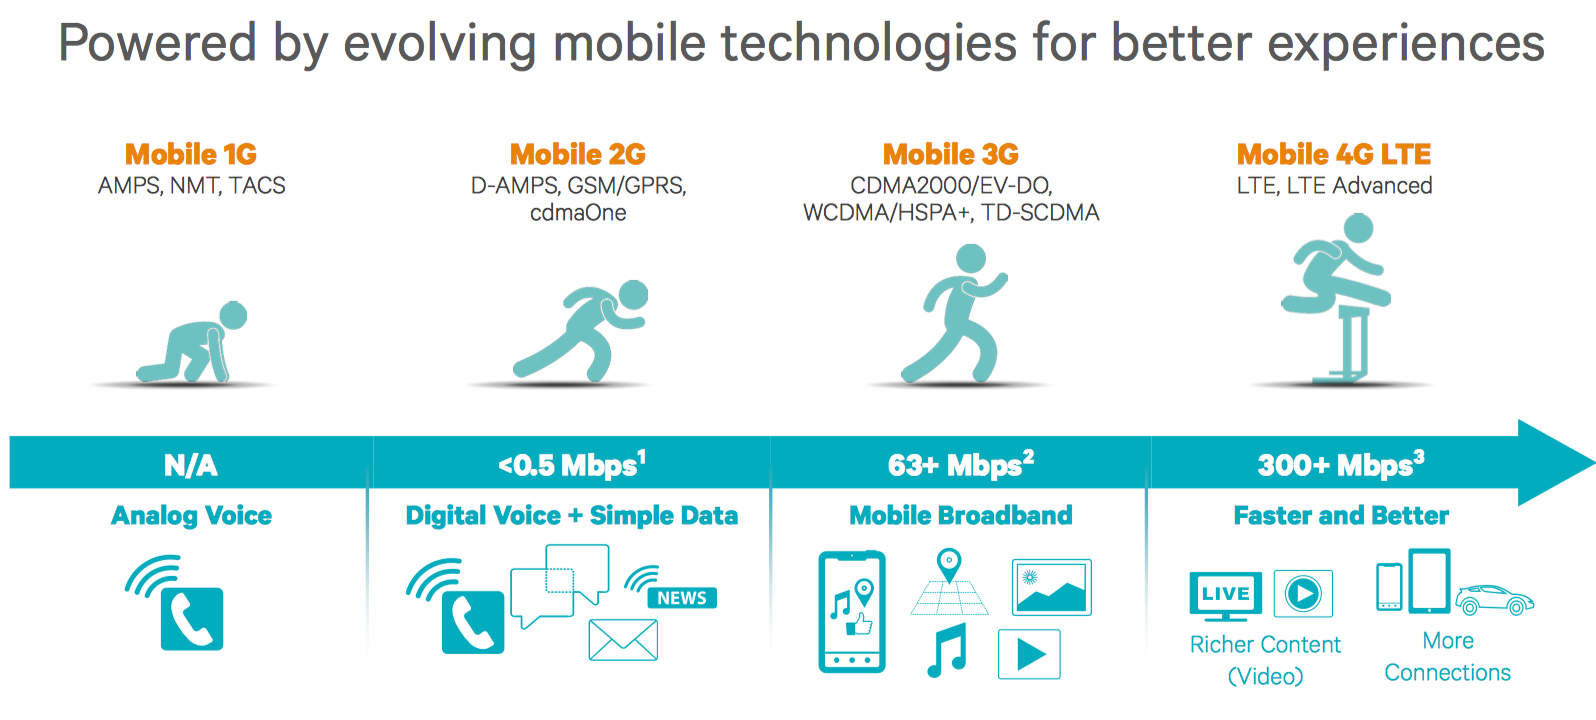
\includegraphics[width=\textwidth]{figures//cellular_speed.png}
    \caption{1G-4G网络的速度对比}
    \end{center}
\end{figure}
3G/4G/5G技术带来的提升可以从以下角度解释
\begin{displaymath}
    C \approx W n \log_{2} (1 + \mathrm{SNR})
\end{displaymath}
$C$是网络容量,$W$波谱范围,$n$是天线个数$\mathrm{SNR}$是信号质量\\
3G/4G/5G通过提供提高更宽的频谱,更多的天线,以及干扰抑制技术来提高网络的容量
\subsection{蓝牙}
\subsubsection{简介}
蓝牙(英语:Bluetooth)。这是一种无线通讯技术标准,
用来让固定与移动设备,在短距离间交换数据,以形成个人局域网(PAN)。
其使用短波特高频(UHF)无线电波,经由2.4至2.485 GHz的ISM频段来进行通信。
1994年由电信商爱立信(Ericsson)发展出这个技术。它最初的设计,
是希望创建一个RS-232数据线的无线通信替代版本。它能够链接多个设备,克服同步的问题。
蓝牙技术目前由蓝牙技术联盟(SIG)来负责维护其技术标准,
其成员已超过三万,分布在电信、电脑、网络与消费性电子产品等领域。
IEEE曾经将蓝牙技术标准化为IEEE 802.15.1,但是这个标准已经不再继续使用。
\subsubsection{蓝牙5.0}
蓝牙5.0在2016年6月被宣布。
在有效传输距离上将是4.2LE版本的4倍(理论上可达300米),
传输速度将是4.2LE版本的2倍(速度上限为24Mbps)。蓝牙5.0还支持室内定位导航功能(结合WiFi可以实现精度小于1米的室内定位),
允许无需配对接受信标的数据(比如广告、Beacon、位置信息等,传输率提高了8倍),针对物联网进行了很多底层优化。
\begin{figure}[H]
    \begin{center}
    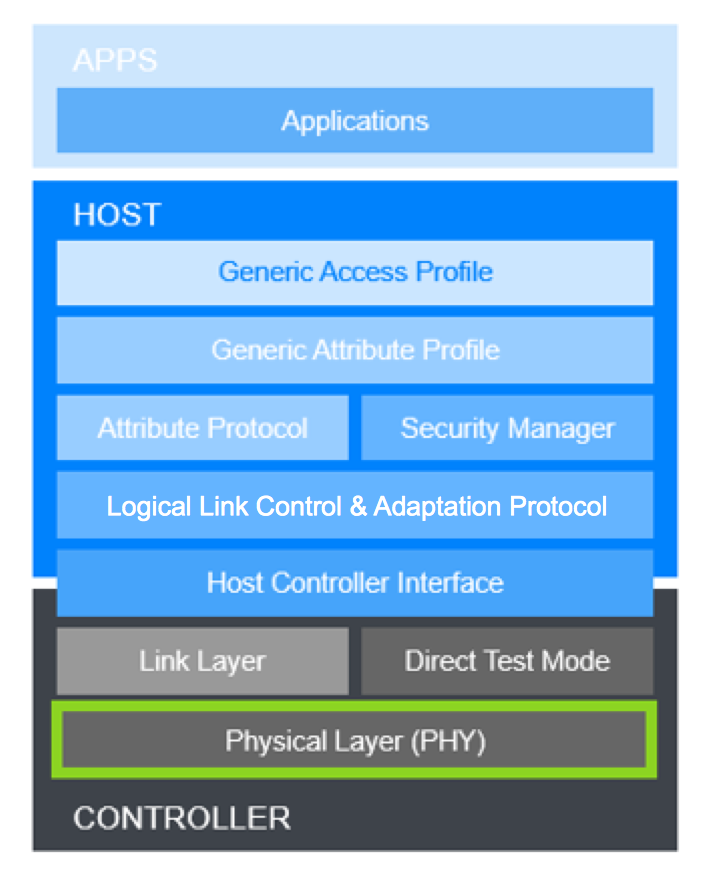
\includegraphics[width=0.67\textwidth]{figures//bluetooth_le.png}
    \caption{蓝牙5.0低功耗版的构架}
    \end{center}
\end{figure}
\subsubsection{性能}
\begin{table}[H]
\begin{center}
\begin{tabular}{cc}
    \toprule
    标准 & 最大速率\\
    \midrule
    Bluetooth 1.0 & 768 Kbps  \\
    Bluetooth 1.1 & 768 Kbps  \\
    Bluetooth 1.2 & 1 Mbps  \\
    Bluetooth 2.0 + EDR & 3 Mbps \\
    Bluetooth 3.0 + HS & 24 Mbps \\
    Bluetooth 4.1 & 24 Mbps \\
    Bluetooth 4.2 & 24 Mbps \\
    Bluetooth 5.0 & 48 Mbps \\
    \bottomrule
\end{tabular}
\caption{蓝牙速度对比}
\end{center}
\end{table}
\begin{figure}[H]
    \begin{center}
    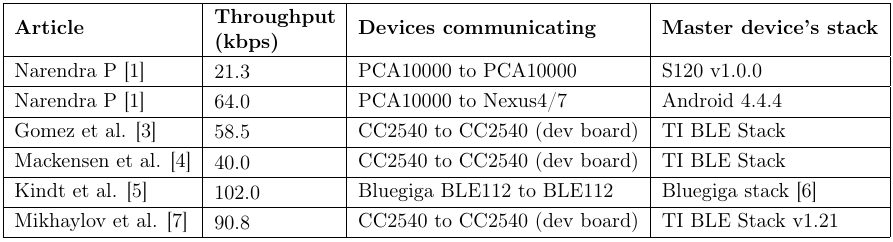
\includegraphics[width=\textwidth]{figures//bluetooth4_speed.png}
    \caption{蓝牙4.0速度的一些测试}
    \end{center}
\end{figure}
\section{立项依据}
\subsection{操作系统同时连接Wi-Fi和Ethernet的情况分析}
现行操作系统中通常是可以同时连接Wi-Fi和Ethernet的,
但如果同时连接Ethernet和WLAN,那么操作系统只会选择其中一个连接使用。
在不修改路由表的情况下,
例如macOS会优先选择拥有用户设置的最高优先级的连接。
而在Windows操作系统中根据跃点数最小的路由来走。
\subsubsection{Windows的网络选择机制}
Windows系统中主要选择了使用度量标准(metric)技术来评估网络质量,
并进行网络选择度量标准是分配给特定网络接口的IP路由的值,
用于标识与使用该路由相关的成本。例如,可以根据链路速度,跳数或时间延迟来评估度量。
自动度量标准是Windows中的一项新功能,
可自动配置基于链接速度的本地路由的度量标准。“自动度量标准”功能默认情况下处于启用状态,还可以手动配置它以分配特定的度量标准。
当路由表包含相同目的地的多个路由时,自动度量标准功能可能很有用。例如,如果计算机具有10Mbps网络接口和100Mbps网络接口,
并且计算机具有在两个网络接口上均配置的默认网关,则自动度量标准功能会将较高的度量标准分配给较慢的网络接口。
例如,此功能可以强制发往互联网的所有流量使用可用的最快网络接口。
\subsection{网卡桥接}
现在为了提高网络吞吐量常有的做法是将两张网卡桥接,
然后通过路由表分配每条链路上的负载,
然而其每个数据服务仍然只能走其中一条链路,
当使用多线程下载工具时,能够实现网速叠加的效果,
然而如果是单个网络服务,比如传送一个视频,其仍然需要分片后手动设置传输的路径,
如果一条数据链路上出错或者连接断开,传输就会出错,而且当一条线路网络条件较差时,
往往会成为传输过程的瓶颈,操作系统并不会为其转换线路后再回到原线路拼接。
\section{重要性、前瞻性分析}
\textbf{使用多路传输文件可以大大增加传输的可靠性}\\
在许多单链路文件传输软件中,经常会有由于链路断开导致文件发送失败的情况,
重新发送有时会从头开始重新传送,大大增加了传送需要的时间。而通过多路传输,
如果一条链路断开,则其他链路保持链接,则传输仍不会停止。
\\
\textbf{能够大大增加文件传输的吞吐量}\\
由于多路传输,可同时利用多路的I/O,速度自然会提升,
由于网络文件传输的瓶颈往往是在网络的I/O上,硬盘读写与CPU的性能不能获得充分利用,
通过多路传输可以更高效利用在文件传输时的硬件利用率。
\\
\textbf{项目的应用前景很广}\\
如果在Linux下实现然后再移植到安卓树莓派等Linux内核的移动端设备上,就能很大提高PC与移动端,移动端与移动端之间的文件传输效率。
而且可以增加优先级定义传输策略,应用在低功耗的物联网设备上,
若同时让它们连上AP主机,再通过蓝牙互相连接,由于蓝牙在距离较远的情况下误码率较高,
丢包可能性也很大,但功耗低,所以在连接状况好时主要通过蓝牙传输,然后在多次丢包或出错后将包交给无线来传输。
\section{相关工作和前沿进展}
\subsection{多路TCP}
\textbf{TODO}
\end{document}